\documentclass[]{article}
\usepackage{lmodern,wrapfig,float}
\usepackage{amssymb,amsmath}
\usepackage{ifxetex,ifluatex}
\usepackage{fixltx2e} % provides \textsubscript
\ifnum 0\ifxetex 1\fi\ifluatex 1\fi=0 % if pdftex
  \usepackage[T1]{fontenc}
  \usepackage[utf8]{inputenc}
\else % if luatex or xelatex
  \ifxetex
    \usepackage{mathspec}
  \else
    \usepackage{fontspec}
  \fi
  \defaultfontfeatures{Ligatures=TeX,Scale=MatchLowercase}
\fi
% use upquote if available, for straight quotes in verbatim environments
\IfFileExists{upquote.sty}{\usepackage{upquote}}{}
% use microtype if available
\IfFileExists{microtype.sty}{%
\usepackage{microtype}
\UseMicrotypeSet[protrusion]{basicmath} % disable protrusion for tt fonts
}{}
\usepackage[margin=0.6cm]{geometry}
\usepackage{hyperref}
\PassOptionsToPackage{usenames,dvipsnames}{color} % color is loaded by hyperref
\hypersetup{unicode=true,
            pdftitle={Alleviating Parking Woes Through ML},
            pdfauthor={Vik Gopal, Achal Rayakar},
            colorlinks=true,
            linkcolor=Maroon,
            citecolor=Blue,
            urlcolor=blue,
            breaklinks=true}
\urlstyle{same}  % don't use monospace font for urls
\usepackage{graphicx,grffile}
\makeatletter
\def\maxwidth{\ifdim\Gin@nat@width>\linewidth\linewidth\else\Gin@nat@width\fi}
\def\maxheight{\ifdim\Gin@nat@height>\textheight\textheight\else\Gin@nat@height\fi}
\makeatother
% Scale images if necessary, so that they will not overflow the page
% margins by default, and it is still possible to overwrite the defaults
% using explicit options in \includegraphics[width, height, ...]{}
\setkeys{Gin}{width=\maxwidth,height=\maxheight,keepaspectratio}
\IfFileExists{parskip.sty}{%
\usepackage{parskip}
}{% else
\setlength{\parindent}{0pt}
\setlength{\parskip}{6pt plus 2pt minus 1pt}
}
\setlength{\emergencystretch}{3em}  % prevent overfull lines
\providecommand{\tightlist}{%
  \setlength{\itemsep}{0pt}\setlength{\parskip}{0pt}}
\setcounter{secnumdepth}{5}
% Redefines (sub)paragraphs to behave more like sections
\ifx\paragraph\undefined\else
\let\oldparagraph\paragraph
\renewcommand{\paragraph}[1]{\oldparagraph{#1}\mbox{}}
\fi
\ifx\subparagraph\undefined\else
\let\oldsubparagraph\subparagraph
\renewcommand{\subparagraph}[1]{\oldsubparagraph{#1}\mbox{}}
\fi

%%% Use protect on footnotes to avoid problems with footnotes in titles
\let\rmarkdownfootnote\footnote%
\def\footnote{\protect\rmarkdownfootnote}

%%% Change title format to be more compact
\usepackage{titling}

% Create subtitle command for use in maketitle
\newcommand{\subtitle}[1]{
  \posttitle{
    \begin{center}\large#1\end{center}
    }
}

\setlength{\droptitle}{-2em}
  \title{\textbf{Alleviating Parking Woes Through ML}}
  \pretitle{\vspace{\droptitle}\centering\huge}
  \posttitle{\par}
  \author{Vik Gopal, Achal Rayakar}
  \preauthor{\centering\large\emph}
  \postauthor{\par}
  \date{}
  \predate{}\postdate{}


\begin{document}
\maketitle

%\abstract{}
{
\hypersetup{linkcolor=black}
\setcounter{tocdepth}{2}
\tableofcontents
}

\section{Introduction}

This report pertains to the following UROPS project:
\begin{quote}
Project number 17165: Application of
Machine Learning Techniques to Automated Parking Lot Classification
\end{quote}
The project is being undertaken by RAYAKAR ACHAL AJEET (A0156139B) in Semester II
of Academic Year 17/18 and is being supervised by Vik Gopal from DSAP. 

The initial task of this project was to train a convolutional neural network
(CNN) to classify images of parking spots\footnote{In this document, an
individual parking space is referred to as a parking \emph{spot}, and spots
constitute a parking \emph{lot}.} from publicly available datasets.  Having
done so, the next part is to apply the techniques we learn to data gathered
within NUS. The purpose of this write-up is to detail this application, with a
focus on how we will protect data gathered within NUS.

The rest of this document is organised as follows: In section
\ref{project-goals}, we summarise the goals of the project. In section
\ref{data-collection-nus}, we outline how we intend to collect the data from
Faculty of Science, and how we intend to protect the data. In the conclusion,
we outline the follow-up work that this project allows us to work on.

\section{Project Goals}
\label{project-goals}

The search for parking spots adds to the tedium of commuting; current
means of expediting search, such as occupancy level billboards outside
parking lots, do not offer sufficiently specific information for the
purpose of finding a spot quickly. We desire to enhance the specificity
of occupancy information available to users through a machine
learning-driven application. Ultimately, we aspire to establish the
following workflow: \newline

\begin{center}
User requests for spot-wise occupancy status through the application, \\
$\downarrow$ \\
Picture of lot taken by a standard CCTV or dedicated camera, \\
and transmitted to associated {\it cloud-based deep-learning model}, \\
$\downarrow$ \\
Spots in picture classified as empty or occupied by model, \\
$\downarrow$ \\
Picture deleted, and user sent spatially-accurate abstraction of spot-wise
occupancy status.
\end{center}

The emphasis is on utilising AI, based on low-cost images of
parking spots, rather than an expensive implementation of sensors at every
parking spot.

\subsection{Choice of Machine Learning
Tool}\label{choice-of-machine-learning-tool}

The deep-learning model aforementioned refers to a convolutional neural
network (CNN). CNNs are a class of artificial neural networks, which are
statistical models that are designed to fit complex nonlinear hypotheses
to data and improve them iteratively and automatically. CNNs in
particular are currently state-of-the-art in computer vision-related
tasks; our task is one of binary image classification.

Before a CNN is ready for use in ascertaining the occupancy of a parking
lot from its picture, it must be trained to do so. This training process
requires a large number of \emph{training examples} -- namely, different
pictures of the parkling lot which each have their spot-wise occupancy
manually labelled. During the training process, the CNN will learn what
aspects of the picture of a spot imply it is occupied or empty through
relating the images to their labels. This training process can take
several hours or days, depending on the number of training examples at
hand.

After training, the CNN will be able to create predictions with an
estimable level of accuracy. Per-image prediction is almost
instantaneous.

\subsection{Partial Proof of Concept}\label{partial-proof-of-concept}

A large dataset concerning two parking lots, PKLot, is available through
\cite{de2015pklot}. The dataset contains about 700,000 images of spots between
the two lots, taken over a month. It is robust in the sense that it contains
images from a wide range of light and weather conditions. Figure
\ref{fig:sample-pklot} contains sample images from these publicly available
datasets.
%\href{https://web.inf.ufpr.br/vri/databases/parking-lot-database/}{is
%publicly available}. The lots are pictured below\footnote{Almeida, P.,
%  Oliveira, L. S., Silva Jr, E., Britto Jr, A., Koerich, A., (2015).
%  PKLot's two parking lots. {[}image{]} Available at:
%  \url{https://web.inf.ufpr.br/vri/databases/parking-lot-database/}
%  {[}Accessed 26 Feb. 2018{]}.}. 

\begin{figure}[H]
  \centering
    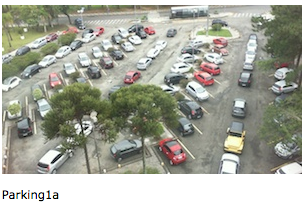
\includegraphics[width=0.3\textwidth]{pklot_1a}
    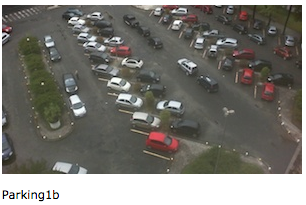
\includegraphics[width=0.3\textwidth]{pklot_1b}
    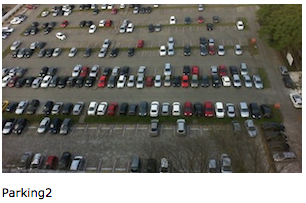
\includegraphics[width=0.3\textwidth]{pklot_1c}
  \caption{Images from publicly available datasets}
  \label{fig:sample-pklot}
\end{figure}

%\begin{center}\includegraphics{writeup_files/figure-latex/unnamed-chunk-1-1} \end{center}
We created a CNN for each of these parking lots, and achieved prediction
accuracies of 99.8+\%, which translated to the misclassification of
about 260 spots in requesting for the prediction of the state of about
175,000. It is therefore without question that CNNs are apt tools for
this task. It will be fruitful to understand how this success can be
replicated in the local context, where we have control over collection
of data.

\section{Data Collection from NUS}
\label{data-collection-nus}

The next phase in our study is to apply the knowledge to the local domain. In
order to do so, we need to collect data from within NUS. This will allow us to
practice the necessary skills to apply a model in practice, starting from data
preparation, cleaning, and thence to model tuning for the specific context.

We initiated a discussion with Sulaiman Salim from the Office of Campus
Amenities (OCA) in order to obtain permission to capture images of parking lots
within NUS. They are interested in the project, and to see how else sensors can
be used to solve other problems that they face, but they
require us to think further about the privacy issues that could arise from
capturing images of parking lots within NUS. The rest of this section details
our proposed data collection procedure, and how we can minimise any intrusion
and exposure of details of individuals and their cars.

\subsection{Equipment, Location, and Frequency of Data Capture}

We intend to use an Arduino Yun (an inexpensive microcontroller board with WiFi
support), connected to a 720p USB webcam and a 64 GB microSD card to capture
pictures of our selected lot. As soon as an image is captured, it will be
encrypted using 256-bit AES (Advanced Encryption Standard) before being
wirelessly uploaded to a private dropbox account.  In addition, the encrypted
version of the image will be written to the microSD for backup purposes. The
encryption helps to protect against malicious individuals who attempt to steal
the data from the physical device, or by hacking it's WiFi account. Regular
logs will inform us if the data is being collected correctly or if something has
gone wrong.
% It is possible to add an IMU to detect motion/tampering and then to secure
% delete the data if tampering is detected. 
% We could even escrow the keys.

After discussing with OCA and doing some scouting of our own, we propose to
perch the device at a vantage point overlooking the parking lot adjacent to
Block S17 and the AYE. Figure \ref{fig:s17-view} an image from the proposed
vantage point, taken at 720p.
%\vspace{4mm}
\begin{figure}[H]
  \centering
    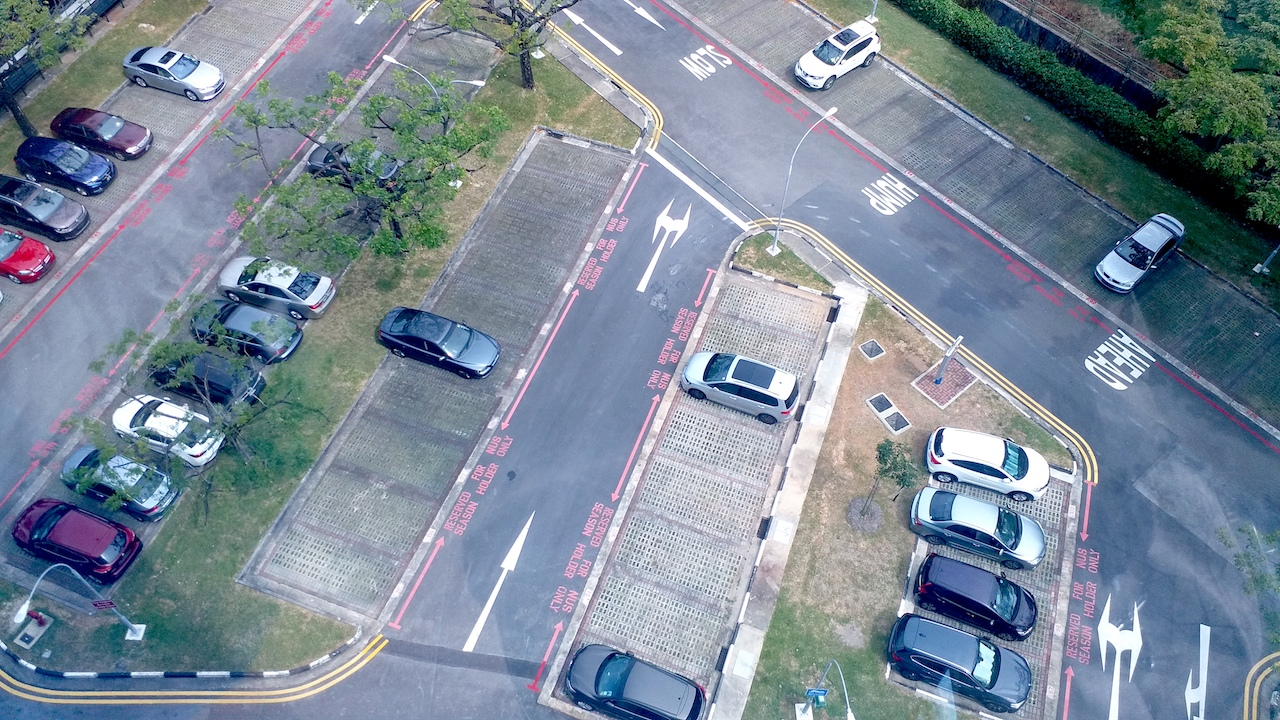
\includegraphics[width=0.6\textwidth]{view_720p}
  \caption{S17 parking lot}
  \label{fig:s17-view}
\end{figure}

The exact location of the vantage point is the highest point of one of the
stairwells in S17. It is explicitly identified by the orange circle in Figure 
\ref{fig:s17_stairwell}
\begin{figure}[H]
  \centering
    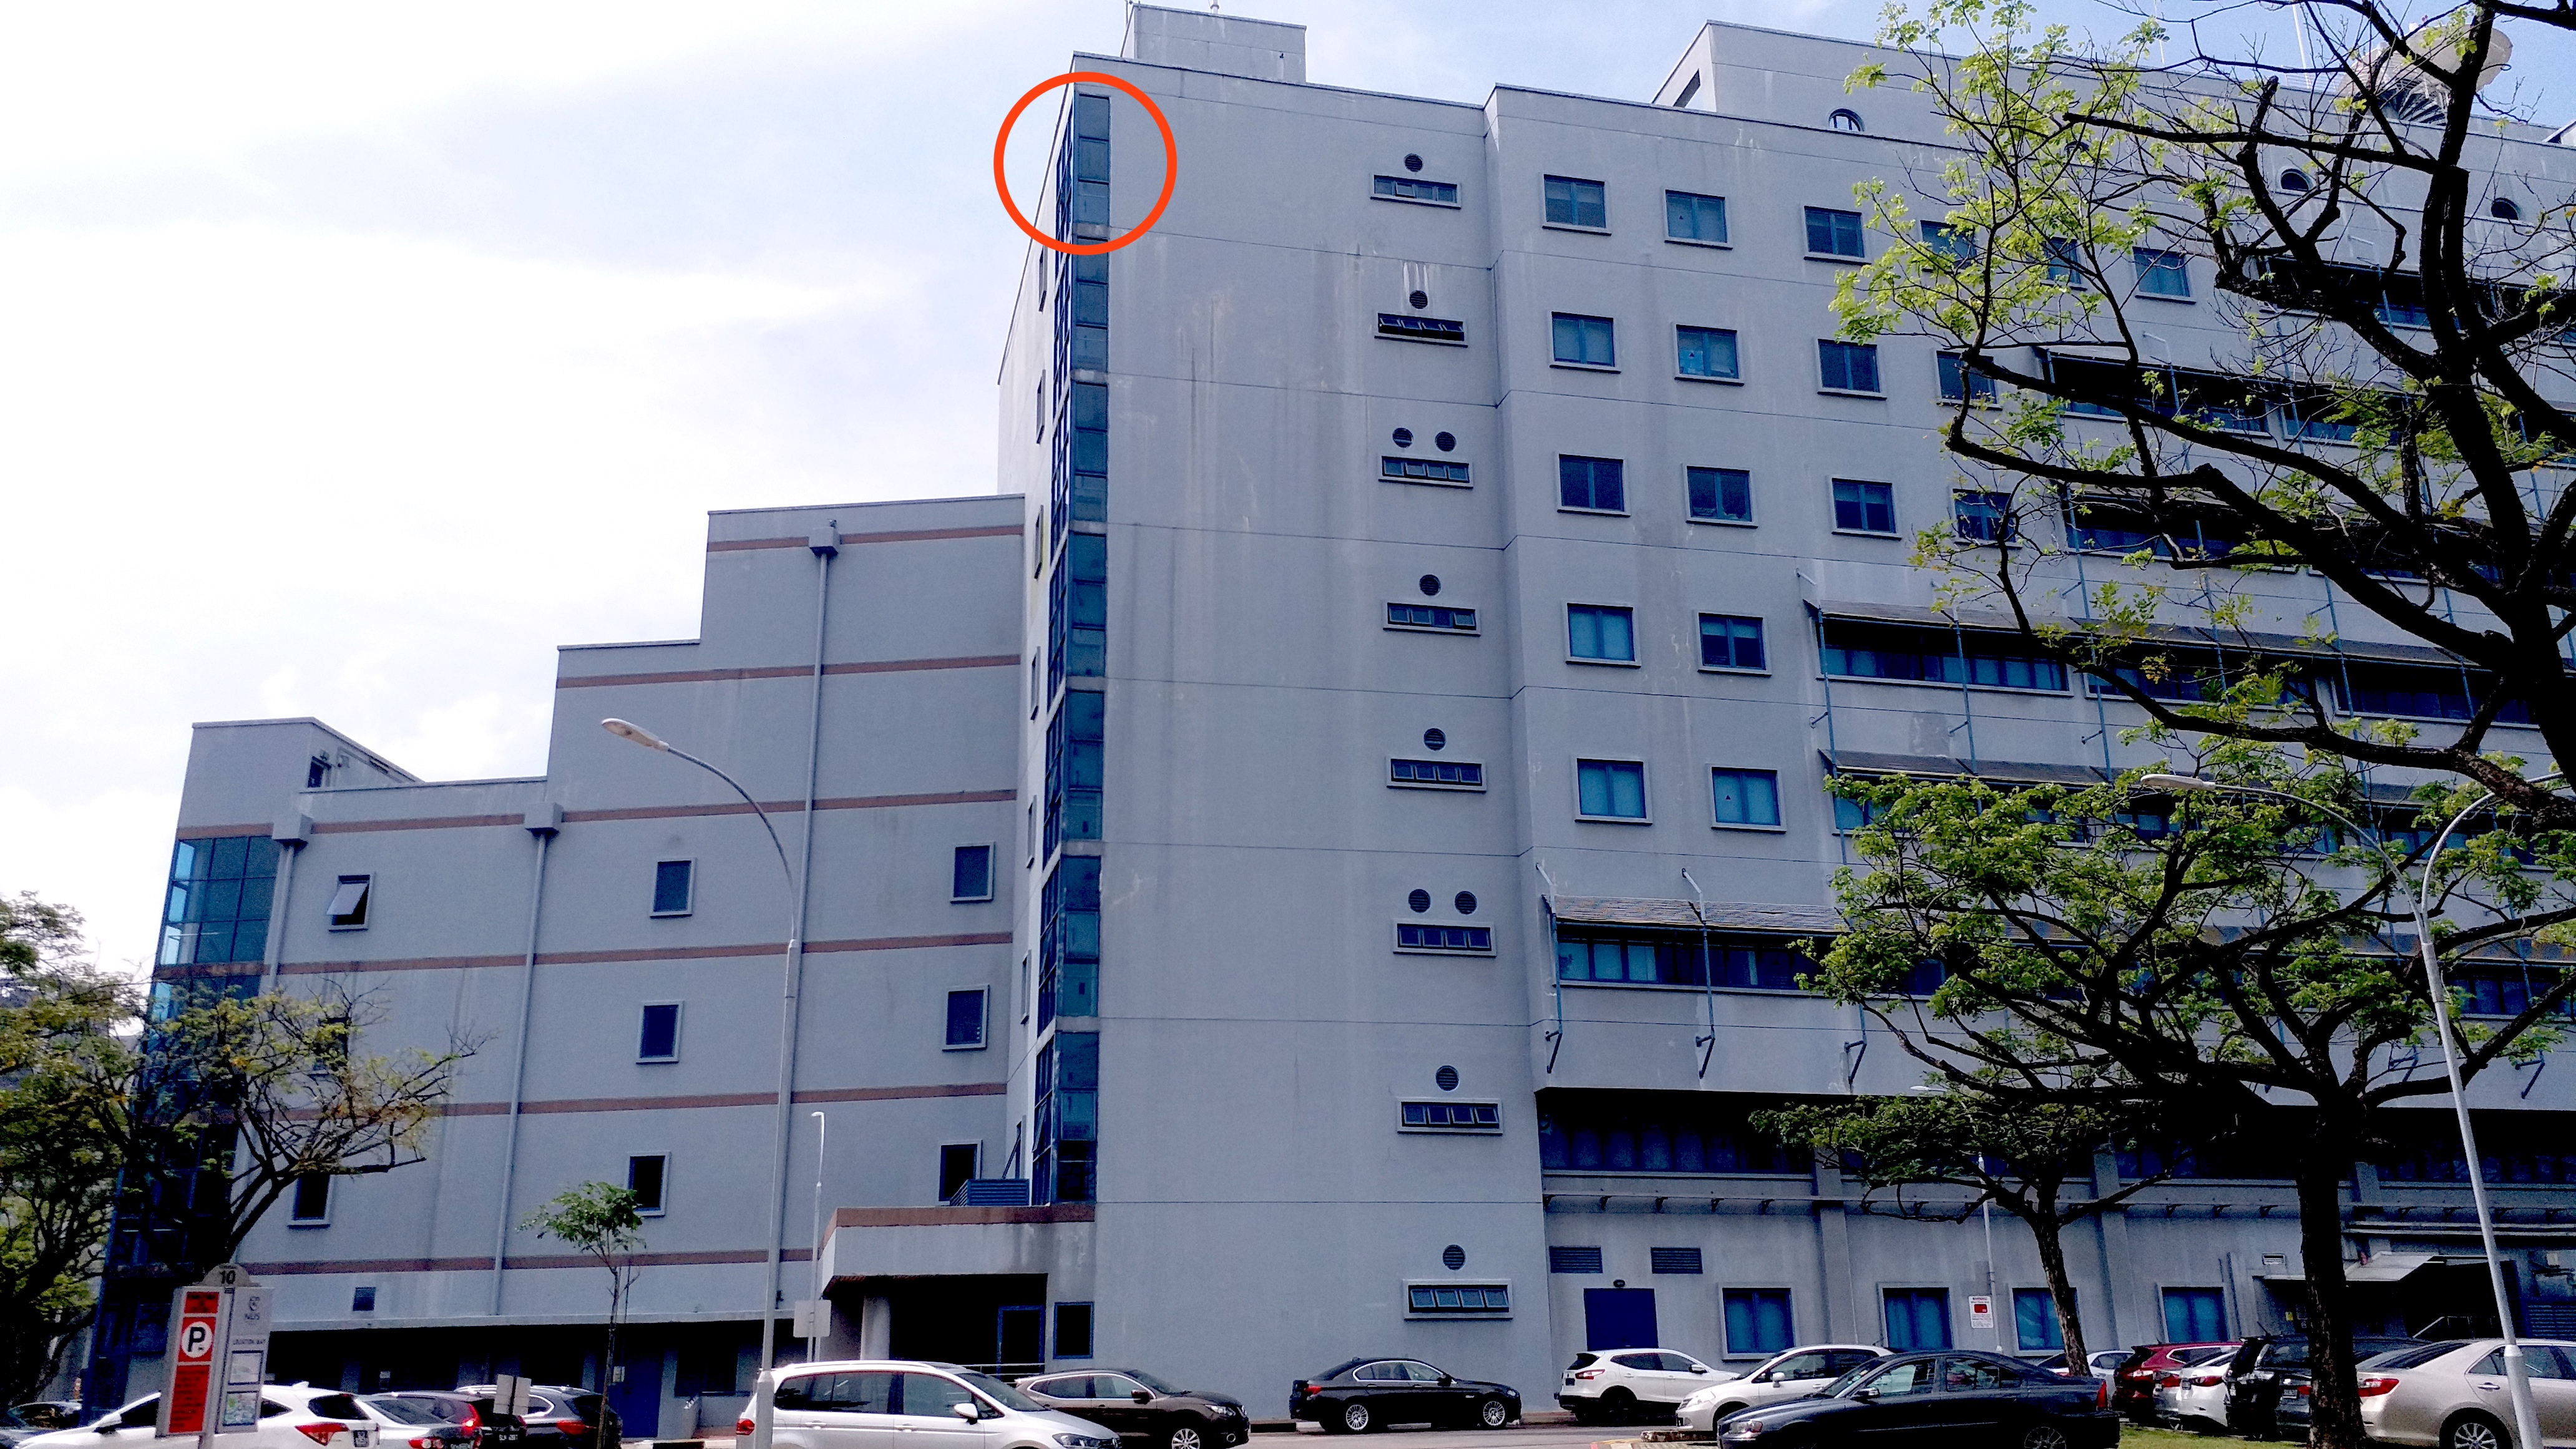
\includegraphics[width=0.6\textwidth]{context2_used}
  \caption{Proposed location of capture device}
  \label{fig:s17_stairwell}
\end{figure}

Judging from the sample pictures taken, the distance and resolution preclude identification
of individual features or humans and identifiable characteristics of cars, such
as their license plates. Thus we believe that the images themselves do not need
to be edited or modified to further safeguard the privacy of individuals.

%\begin{center}\includegraphics{writeup_files/figure-latex/unnamed-chunk-2-1} \end{center}\newpage
%Some context of the vantage's location:
%\begin{center}\includegraphics{writeup_files/figure-latex/unnamed-chunk-3-1} \end{center}
%\begin{center}\includegraphics{writeup_files/figure-latex/unnamed-chunk-3-2} \end{center}

We propose to obtain approximately 200,000 images of parking spots. This is of
the same order as the publicly available dataset, and is what allowed us to
achieve the observed level of accuracy. Based on the number of parking spots
in the images above (approximately 50), we would be able to achieve our target
if we capture images at five minute intervals, every daylight hour, for four
weeks. 

%Images will be taken by the device at five minute intervals for most of
%the working day, for four weeks. They will be
%\href{https://learn.adafruit.com/wireless-security-camera-arduino-yun/introduction}{wirelessly
%transmitted to a private DropBox account}, and will also be encrypted
%and stored in the attached microSD card for backup purposes.
%
When the observational period is over, all images will be downloaded and
then secure deleted from the microSD card and DropBox account. 
%Before further
%use, they will be processed:
%
%\emph{(An aside)} privacy concerns regarding identifiable features of
%licence plates and persons. Given the resolution of the camera, and the
%distance and angle of the vantage from the lot, little has to be done to
%obscure such features. Therefore it will be sufficient to apply a light
%blur to images before storage: \vspace{4mm}
%
%\begin{center}\includegraphics{writeup_files/figure-latex/unnamed-chunk-4-1} \end{center}
%
\subsection{Training the CNN, in the Cloud.}\label{training-the-cnn-on-the-cloud.}

Training and configuration of CNNs will be done online on
\href{https://www.floydhub.com}{Floydhub}, which means that we will ultimately
be storing all collected image data on a private repository on the cloud. These
images will stay there until this project culminates, likely in August 2018.
There are a number of reasons for these choices:

\begin{enumerate}
  \item The Python machine learning library that we use, TensorFlow, is set up
and updated automatically for us on FLoydhub along with all dependency modules.
  \item Great computing power is available on the cloud inexpensively; it will
  save us many hours in training.
  \item Training multiple configurations of the same CNN concurrently is
  possible -- on a personal computer, it is not. Again, time will be saved.
  \item Working on the cloud allows all involved in the project to collaborate
  seamlessly, and is the norm in industry.
  \item Moving development to the cloud will better prepare us to serve the
model to users in future.
\end{enumerate}

We have queried Floydhub regarding their security practices in order to satisfy
our concerns that it could be a point of weakness in our workflow.  Floydhub is
hosted on AWS; they too use 256-bit AES to communicate with local machines to
run jobs. They have taken measures to restrict the number of users (to just
two) who have administrative access to their servers. Finally, user passwords
and authentication tokens are not managed by them, but by Auth0. We believe
this is more than sufficient for our application and data.

%\subsection{Responding to User Requests, on the
%Cloud.}\label{responding-to-user-requests-on-the-cloud.}
%
%Tools like
%\href{https://aws.amazon.com/blogs/machine-learning/how-to-deploy-deep-learning-models-with-aws-lambda-and-tensorflow/}{Amazon's
%Amazon Web Services} (AWS) allow us to put a CNN on the cloud for
%prediction purposes. They offer serverless services that can scale
%dynamically in capacity in response to demand, and are only billed per
%user request. Our application intends to harness this tool in its
%back-end.

\section{Conclusion and Extensions}\label{conclusion}

Increasing the resolution of information available to those seeking a
parking spot is not the only implication of this project, especially
given that NUS' parking lots are organized appropriately for demand.
Rather, we truly view this project as a capability-building exercise; a segue
into greater problems that can be addressed by machine learning --
either by us or those who take reference to our experiences in the
future. For instance, even in the context of this application, there are
several extensions that we could consider:
\begin{enumerate}
\tightlist
\item How well can we classify the lots using grayscale images, which is
typically what we obtain from CCTV cameras?
\item How well can we classify lots at night?
\item How can we overcome occlusion due to trees or neighbouring large cars?
\item How well can the model perform this task indoors? How extensive a network
of cameras would be needed in such a case?
\end{enumerate}

\bibliographystyle{plain}
\bibliography{ref}


\end{document}
